\documentclass[a4paper]{article}
\usepackage{mathtools}
\DeclarePairedDelimiter\ceil{\lceil}{\rceil}
\usepackage{graphicx}
\title{adolescence}
\author{Dymitr Lubczyk \and Wojciech Replin \and Bartosz Różański}


\begin{document}
	\maketitle
	\begin{abstract}
		Some generic abstract
	\end{abstract}
	
	\newpage
	\section{Implemented Algorithms}
	\subsection{Elimination Tree Data Structure}
	Elimination Tree proved to be a central figure in many of algorithms that we implemented. It is an implementation of Treedepth decomposition of incomplete elimination defined in introductory documentation, thus we will mention it briefly here:
	\begin{enumerate}
		\item Treedepth decomposition of incomplete elimination $w$ is a rooted tree $T_w$ such that:
		\begin{itemize}
			\item Treedepth decomposition of empty elimination (empty word $\varepsilon$) is a single vertex represented by $G$.
			\item Treedeph decomposition of incomplete elimination $wv$, is built from $T_w$, in the following way:
			\begin{enumerate}
				\item Find leaf $H$ in $T_w$ such that $v\in H$.
				\item Add every connected component of $H-v$ as a child of $H$.
				\item Replace node $H$ with $v$.
			\end{enumerate}
		\end{itemize}
		\item Depth of a node $v$ in $T_w$ is defined as a length of a path between $T_w$ root and $v$ and is denoted as $depth_{T_w}\left(v\right)$.
	\end{enumerate}
	Its implementation can be found in \texttt{elimination\_tree.hpp}.
	\subsection{Heuristics}
	\subsubsection{Highest Degree Heuristic}
	The idea behind this heuristic is pretty simple and came naturally. The vertices with higher degree are more likely to be higher in a best tree decomposition. To get tree depth decomposition we use the recursive definition.
	\begin{equation}
	td\left(G\right) = 
	\begin{cases}
	1, & \mbox{if}\left|G\right|=1 \\
	1+\min_{v\in V}td\left(G-v\right) & G\mbox{ is connected and }\left|G\right| > 1 \\
	\max _i td(G_i) & \mbox{otherwise} \\
	\end{cases}
	\label{tddef}
	\end{equation}
	the equation above expresses the idea of removing vertices in order to get tree depth decomposition. The procedure of computing tree depth decomposition can be easily expressed with Elimination Tree data structure mentioned before:
	\begin{enumerate}
		\item Initialize Elimination tree $t$ with $G$.
		\item As long as there is component $C$ in $t$ select and then remove vertex from $C$.
	\end{enumerate}
	The result of this algorithm will be tree decomposition of $G$ stored in $t$. So the highest degree heuristic goes as above, but it always selects vertex $v$ with the highest degree in $C$. More specific analysis of this heuristic will be presented in following sections, but important thing is that it has time complexity $O(n^2)$ and gives decent results for dense graphs.
	\subsubsection{Variance Heuristic}
	In this algorithm we use the same procedure to generate tree decomposition of $G$ as in previous section, but the selection of $v$ to be removed in $C$ is slightly different. We will mark set of components achieved by removing $v$ from $C$ as $C_v$ and variance of size of elements in this set as $\sigma^2(C_v)$. We will choose vertex which maximizes: 
	\begin{equation}
	\frac{\alpha}{\sqrt{\sigma^2(C_v)+\gamma}}+\beta\cdot |C_v|
	\end{equation}
	where $\alpha$, $\beta$ and $\gamma$ are constants determined empirically (currently parameters $\alpha=0.2$, $\beta=0.8$ and  $\gamma=1.0$ produced the best results yet). In case of a draw, we choose vertex with higher degree. This approach works better than Highest Degree Heuristic in almost all cases. It is worth mentioning that it works very well for sparse graphs, especially for trees. Time complexity of this algorithm is $O(n^3)$, the further analysis will be provided later on.
	\subsubsection{Bottom-Up Heuristic}
	This approach trades off space complexity of $O^*\left(2^n\right)$ for time complexity of  $O^*\left(2^n\right)$ and fairly good approximations. We shall incorporate a Union-Find data structure to represent components of induced subgraph. We will add one vertex at a time to every known induced subgraph. We distinguish induced subgraphs by their depth, and keep ones that have it the smallest. This algorithm does not produce exact solutions, as much as we would hope it did, because we do not optimize choice of vertex for components which this vertex would connect. We do not know how bad of an approximation this algorithm can produce (probably as bad as it gets), but for as long as we had memory to keep it running it was not far off from the optimal solutions. In fact, it produces optimal solutions so often, we almost accepted this algorithm as an exact one. During our testing, it produced solutions not worse than 2(!) deeper than the optimal one. We implemented it on a GPU and its implementation can be found in \texttt{bottom\_up\_heuristic\_gpu\_algorithm.hpp}.
	\subsection{Lower Bounds}
	\subsubsection{Lower Bound from number of edges}
	We have discovered a function which for given graph $G=(V,E)$ tells us what is a minimum treedepth value for this graph:
	
	\begin{equation}
	f(n,e)=\ceil*{\frac{1}{2}+n-\sqrt{\frac{1}{4}-n+n^2-2e}}
	\end{equation}
	\\Here is our thought process.
	Let us look at this problem from opposite direction. Given a particular treedepth decomposition, we can create from it all graphs for which this decomposition will be valid. This is pictured on the figure below. As we can see, the treedepth decomposition on the left is a valid decomposition for any graph which has some of the edges shown on the right as a dotted lines. Or in other words: is a valid decomposition for graph on the right and all graphs induced by it. %this sentence is not correct in this context, CHECK INDUCED GRAPH DEFINITION
	\begin{center}
		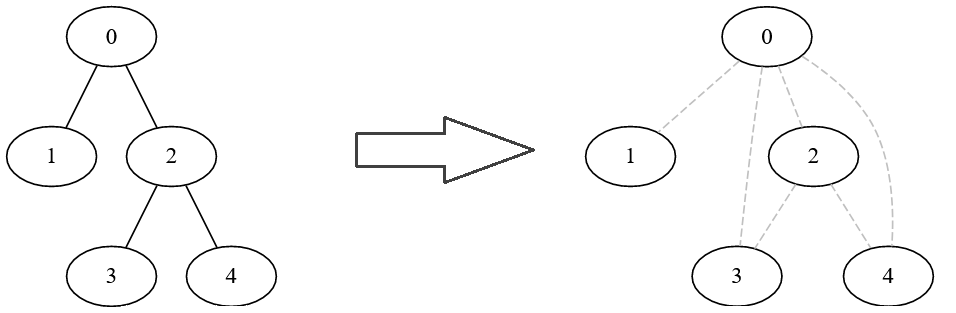
\includegraphics[width=\textwidth]{transform.png}
	\end{center}
	Here we can notice an important thing: a vertex on level $k$ adds $k-1$ edges that input graph can possibly have. In this example, vertex 3 creates two additional edges that a potential input graph can have: edge 3-0 and 3-2, while vertex 2 - being on level 2 - creates only one additional edge (2-0).\\ 
	%This is not very precise
	% This should be Spain sth like this:
	% Let us notice, that a vertex on level k>0 can be a neighbour of maximum of k-1 of its descendants
	Knowing this we can ask ourselves a question: having a fixed treedepth value $td$ and fixed number of vertices $n$, what the structure of treedepth decomposition ,that maximizes number of possible edges in input graph, might look like?\\
	Let us carry out the following construction. We start with $n$ vertices and no edges.
	At the beginning we do not have any choice as we have to ensure that $td$ equals given value, so we construct $P_{td}$ path. Now we are still left with $n-td$ vertices - where should we attach them to maximize the number of possible edges in input graph? As we have said earlier: a vertex on level $k$ adds $k-1$ edges that input graph can possibly have. From this we conclude that we have to attach in such a way that they will be on the lowest possible level which in our case is $k=td$. Below is an example for $td=3$ and $n=5$.
	\begin{center}
		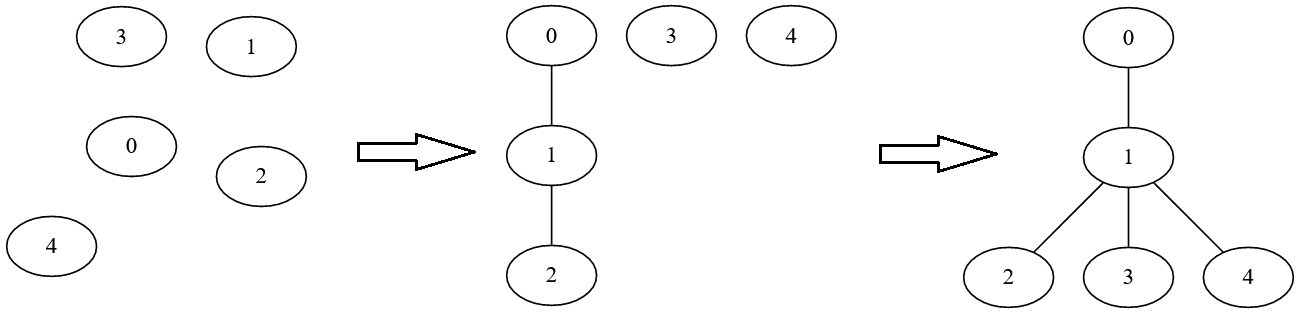
\includegraphics[width=\textwidth]{construction.png}
	\end{center}
	From all treedepth decompositions with fixed $td$ and $n$, this one supports the highest possible number of edges in input graph. This decomposition supports maximally up to
	$$\sum\limits_{i=1}^{td-1} i + (n-td)(td-1)$$edges. The sum part of equation corresponds to the $P_{td}$ path and rest of the equation takes for account the vertices which we attach at the lowest level.\\
	Finally, solving this equation for $td$ leaves us with formula presented at the beginning.
	\clearpage
	\subsection{Exact Algorithms}
	\subsubsection{Iterative Dynamic}
	This is first algorithm we figured out when we started reading about tree-depth problem. We are going to iterate over $k$, from $1$ to $|G|$ and for every $S\subseteq V(G)$ such that $|S|=k$ we are going to: 
	\begin{enumerate}
		\item If graph induced on $S$ is disconnected go to next subset
		\item Else for every $v\in S$ store $td(G[S\backslash v])$ as treedepth of the highest component of $G[S\backslash v]$
		\item As the depth of $G[S]$ take the smallest $td(G[S\backslash v])$ plus $1$.
	\end{enumerate}
	Note that step 2 reaches into results calculated in previous iterations, hence the name Dynamic Algorithm.\\
	As we can see this algorithm generates cache with tree depth and root of best tree depth decomposition for every connected induced subgraph of $G$. As we go from smaller subsets to bigger, there are always stored results for components of $G[S\backslash v]$ because they are smaller than size of subset, we are working on. The pessimistic complexity of this algorithm is $O(n^2 \cdot 2^n)$. The difference is pretty small for different graphs, but in general it performs better for sparse one.
	\subsubsection{Recursive Dynamic}
	In contrary to iterative dynamic algorithm, we shall calculate treedepth of a graph in a recursive manner, which better illuistrates the idea behind the definition of treedepth.\\
	It shares some features with a iterative approach:
	\begin{enumerate}
		\item Whenever we successfully calculated treedepth of a graph, we save that information for later to avoid repeating calculations
		\item We keep treedepth information only about connected graphs
	\end{enumerate}
	On the other hand this approach enables some optimizations which are not suitable for iterative approach:
	\begin{enumerate}
		\item Graph encoding can be changed for faster binary encoding since we do not rely on optimality of set encoding
		\item Elimination Tree data structure is used to detect connected components of induced subgraph which avoids recalculation of such components and is more efficient overall
	\end{enumerate}
	Sadly, binary encoding limits number of vertices of a graph to be processed. Currently it is set to 128 but easily expandable to up to 1024.\\
	Implementation of this algorithm can be found in \texttt{dynamic\_cpu\_improv.hpp}.
	\newpage
	\subsubsection{Raw Branch and Bound}
	This algorithm is a fairly straight-forward branch and bound algorithm, but includes few problem-specific optimizations. It uses Elimination Tree data structure in order to keep track of components yet to be eliminated:
	\begin{enumerate}
		\item If set of connected components is empty, update current solution if necessary
		\item For every connected component, test whether current branch should be pruned based on a lower bound on treedepth for this component
		\item For every vertex $v$ from the first connected component, traverse subtree rooted in $v$
	\end{enumerate}
	Differences from standard B\&B include:
	\begin{enumerate}
		\item Elimination order of vertices from different components is not differentiated. This results in every set of components to be eliminated to be considered exactly once during the execution of this algorithm
		\item Lower bounds are calculated for every connected component independently
	\end{enumerate}
	And their significance:
	\begin{enumerate}
		\item This modification granted us massive increase in performance basically for free due to an easy access to each connected component
		\item This modification simplified implementation of lower bound algorithms and allows us to tell quicker whether a branch should be pruned. It also allows us for some parallelism but it is yet to be implemented
	\end{enumerate}
	Overall performance of this algorithm shall be discussed later. Implementation of this algorithm can be found in \texttt{branch\_and\_bound.hpp}.
	\subsubsection{Branch and Bound with Cache}
	Go to 1.4.2
	\newpage
	\section{Data Analysis}
\end{document}
